\chapter{ Introduction }

\label{introduction:introduction}

% Purpose:
%\begin{itemize}
%   \item A. Section overview
%   \item B. Why you should read this manual
%   \item C. How to use this manual
%   \item D. Terminology
%   \item E. Overview of library
%   \item F. Program control
%   \item G. Error messages
%   \item H. Section summary
%\end{itemize}
%\begin{center}
%*********************  \newline
%\end{center}
%\vspace{0.25in}

% Quote:
% The successful con artist is a mirror of the time and place where he works.

%\textcolor{red}{ROSE}


\section{What is ROSE}

% Describe ROSE to the broad target audience.
% Describe how it works 
%    Read the input source code
%    Generate the AST (define AST and define graph) 
%       The structure of the original source code is preserved
%       Details aboaut the source code can be found in the AST
%    Provide tools 
%       for the analysis and transformation of the AST
%       generate additional information from the AST (call graph, etc.)
%       visualization of the program
%    Source code regneration
%       
% 
   ROSE is an open source compiler infrastructure for building tools that can
read and write source code in multiple languages (C/C++/Fortran)
and/or analyze binary executables in (x86, Power-PC, and ARM).
The audience for ROSE is people building tools for the analysis
and transformation of source code and/or analysis of binary 
executables.  ROSE provides a library (librose) that can be 
used to support the universal requirements of tools that
do custom analysis and or transformations on software. 

   ROSE works by providing the infrastructure support to
user-defined tools so that they need not implement the 
complex support required for for common operations. 
For source code based tools these include parsing, common forms of 
compiler analysis, common transformations, and code generation.
For binary analysis based tools these include disassembly,
function boundary detection, common forms of analysis.
User defined tools may also mix source code and binary analysis
to form more interesting tools for specialized purposes.
ROSE is part of research work to unify the analysis of
both source code and binaries within general compiler research.

   ROSE works by reading the source code and/or binary
and generating an Abstract Syntax Tree (AST).  The AST forms
a graph representing the structure of the source code and/or binary
executable and is held in memory to provide the fastest possible means 
of operating on the graph.  The nodes used to define the AST graph are 
an {\em intermediate representation} (IR) common within compiler research
as a way of representing the structure of software absent syntax details
(commas, semi-colons, white-space, etc.).  ROSE provides mechanisms to 
traverse and manipulate the AST. Finally, in the case of source code, 
ROSE provides a mechanisms to regenerate source code from the AST.

   As a trivial example, if the input source code program contains a variable declaration
for an integer, all of this information will be available in the AST.
Similarly, an automated transformation of the variable declaration 
held in the AST would be expressed in source code regenerated from the 
AST.  In the case of binaries, (including executables, object files, and libraries)
the AST will represent the structure of the binary, including the 
binary file format (symbol table, debug format, import tables, etc.), 
disassembled instructions, all instruction operands, etc.

  ROSE provides a rich set of tools to support the analysis of 
software including the support for users to build their own forms
of analysis.  A wide assortment of AST traversals are provided
to express both analysis and transformations of the AST. A set of
common forms of analysis are provided (call graph, control flow, etc.)
most work uniformly on both source code and binary executables.
Visualization support in included to help users understand and debug
their tools.  GUI support is available to support building professional
level tools using ROSE. ROSE is actively supported by a small
group at LLNL and is used as a basis for compiler research work within 
DOE at LLNL.


% Sections suggested by Carol Eidt (at Microsoft)
\section{Why you should be interested in ROSE}

ROSE is a tool for building source-to-source translators.
You should be interested in ROSE if you want to 
understand or improve any aspect of your software. ROSE
makes it easy to build tools that read and operate on source code
from large scale applications (millions of lines).  Whole projects
may be analyzed and even optimized using tools built using ROSE.

\section{Problems that ROSE can address}
    ROSE is a mechanism to build source-to-source analysis or 
optimization tools that operate directly on the source code of large 
scale applications.  Example tools that {\em have} been built include:
\begin{itemize}
   \item Array Class abstraction optimizer,
   \item Source-to-source instrumenter,
   \item Loop analyzer,
   \item Symbolic complexity analyzer,
   \item Code coverage tools,
   \item and many more.
\end{itemize}
Example tools that {\em can} be built include:
\begin{itemize}
   \item Custom optimization tools,
   \item Custom documentation generators,
   \item Custom analysis tools,
   \item Code pattern recognition tools,
   \item Security analysis tools,
   \item and many more.
\end{itemize}


\section{Research Goals for ROSE}
ROSE is a project that aims to define a new type of compiler technology that allows
compilation techniques to address the optimization of user-defined abstractions.
Due to the nature of the solution we provide, it is also an open compiler infrastructure
that can be used for a wide number of other purposes.

   User-defined abstractions are built from within an existing base language and
carry specific semantic information that can't be communicated to the base
language's compiler.  In many situations, the semantic information could be useful within
program optimization, but the base-language compiler is forced to ignore this semantic 
information because there is no way for applications to pass such additional information 
to the base-language compiler. Note that {\tt \#pragmas} only permit information that the 
base-language compiler might anticipate (expect) to be passed; it is not a meaningful 
mechanism to communicate arbitrary information about user-defined abstractions to a 
compiler.  ROSE is a part of general research on {\em telescoping languages} (a term 
coined by Ken Kennedy at Rice University) and CELL languages (a term coined by 
Bjarne Stroustrup).  It is part of general work to define domain-specific languages
economically from general purpose languages.

\fixme{Check spelling of CELL in recent work by Bjarne}

\section{ROSE: A Tool for Building Source-to-Source Translators}

   ROSE represents a tool for building source-to-source translators.
Such translators can be useful for many purposes:
\begin{itemize}
   \item automated analysis and/or modification of source code
   \item instrumentation
   \item data extraction
   \item building domain-specific tools
\end{itemize}
An optimizing translator can be expected to both analyze the input 
source code and automatically generate transformations of the source code; the
result being a new source code. If successful, the automatically generated source 
code will demonstrate better performance.  ROSE is the tool that helps users write
such source-to-source translators.  Expected users would be library writers and
tool developers, not necessarily the application developers.  As a result, we expect
the ROSE user to be more knowledgeable about programming languages issues than the 
average application developer.

ROSE translators are particularly useful as a way to bridge the gap between what we want
compilers to do and what they actually do.  This {\em semantic gap} is significant when
optimizing user-defined abstractions (functions and/or data structures), because the
base-language compiler has no knowledge of their semantics.  The optimization
is particularly important within scientific applications.  Such applications are often
expensive to build because they are exceedingly complex and must too often be
written at low levels of abstraction to maintain significant performance on
modern computer architectures.  The modern computer architectures themselves also
vary widely and make the optimization of software difficult.

\section{Motivation for ROSE}

   The original motivation for the development of ROSE comes from work within the Overture Project
to develop abstractions for numerical computation that are efficient and easy to use.
Basically, C++ language mechanisms made the abstractions easy to use (if not tedious to
build), but efficiency was more problematic since the optimization of low-level
abstractions can be (and frequently is) not handled well by the compiler.  Specifically
the rich semantic information the library writer embeds into his abstractions can't
be communicated to the compiler, so many optimizations are missed.  ROSE has addressed
this fundamental problem by simplifying how an optimized translator could be built and
tailored to a library's abstractions to introduce optimizations that use the high-level 
semantics of user-defined abstractions.

\section{ROSE as a Compiler Framework}

    ROSE contains compiler infrastructure. This is because a translator that reads
source code in any language is essentially a compiler (or {\em translator}).  The most precise understanding
of a source code in any language is the process of compiling it.  Source-to-source
compilation can, however, skip the common back-end code generation (since source code is
generated instead of object code in the form of an executable).  ROSE translators
pay particular attention to reconstruct the generated source code (including comments and
CPP translator control directives [\#include, \#if, \#else, \#endif, etc.], and 
the original application's indentation and variable names, etc.).

    ROSE is unique because 
% What is different about ROSE is that 
it makes traditional compiler infrastructure
accessible to library and tool developers who are not likely to have a significant compiler
background.  Still, some basic knowledge of an Abstract Syntax Tree (AST) is 
assumed (and, unfortunately, currently required).  
% In future work we will continue to simplify what is presently required background, as much as possible.

   Figure \ref{introduction:phases} shows the different phases of processing within ROSE.

\begin{figure}
%\centerline{\epsfig{file=rose-processing-phases.ps,height=1.0\linewidth,width=1.0\linewidth,angle=0}}

%\centerline{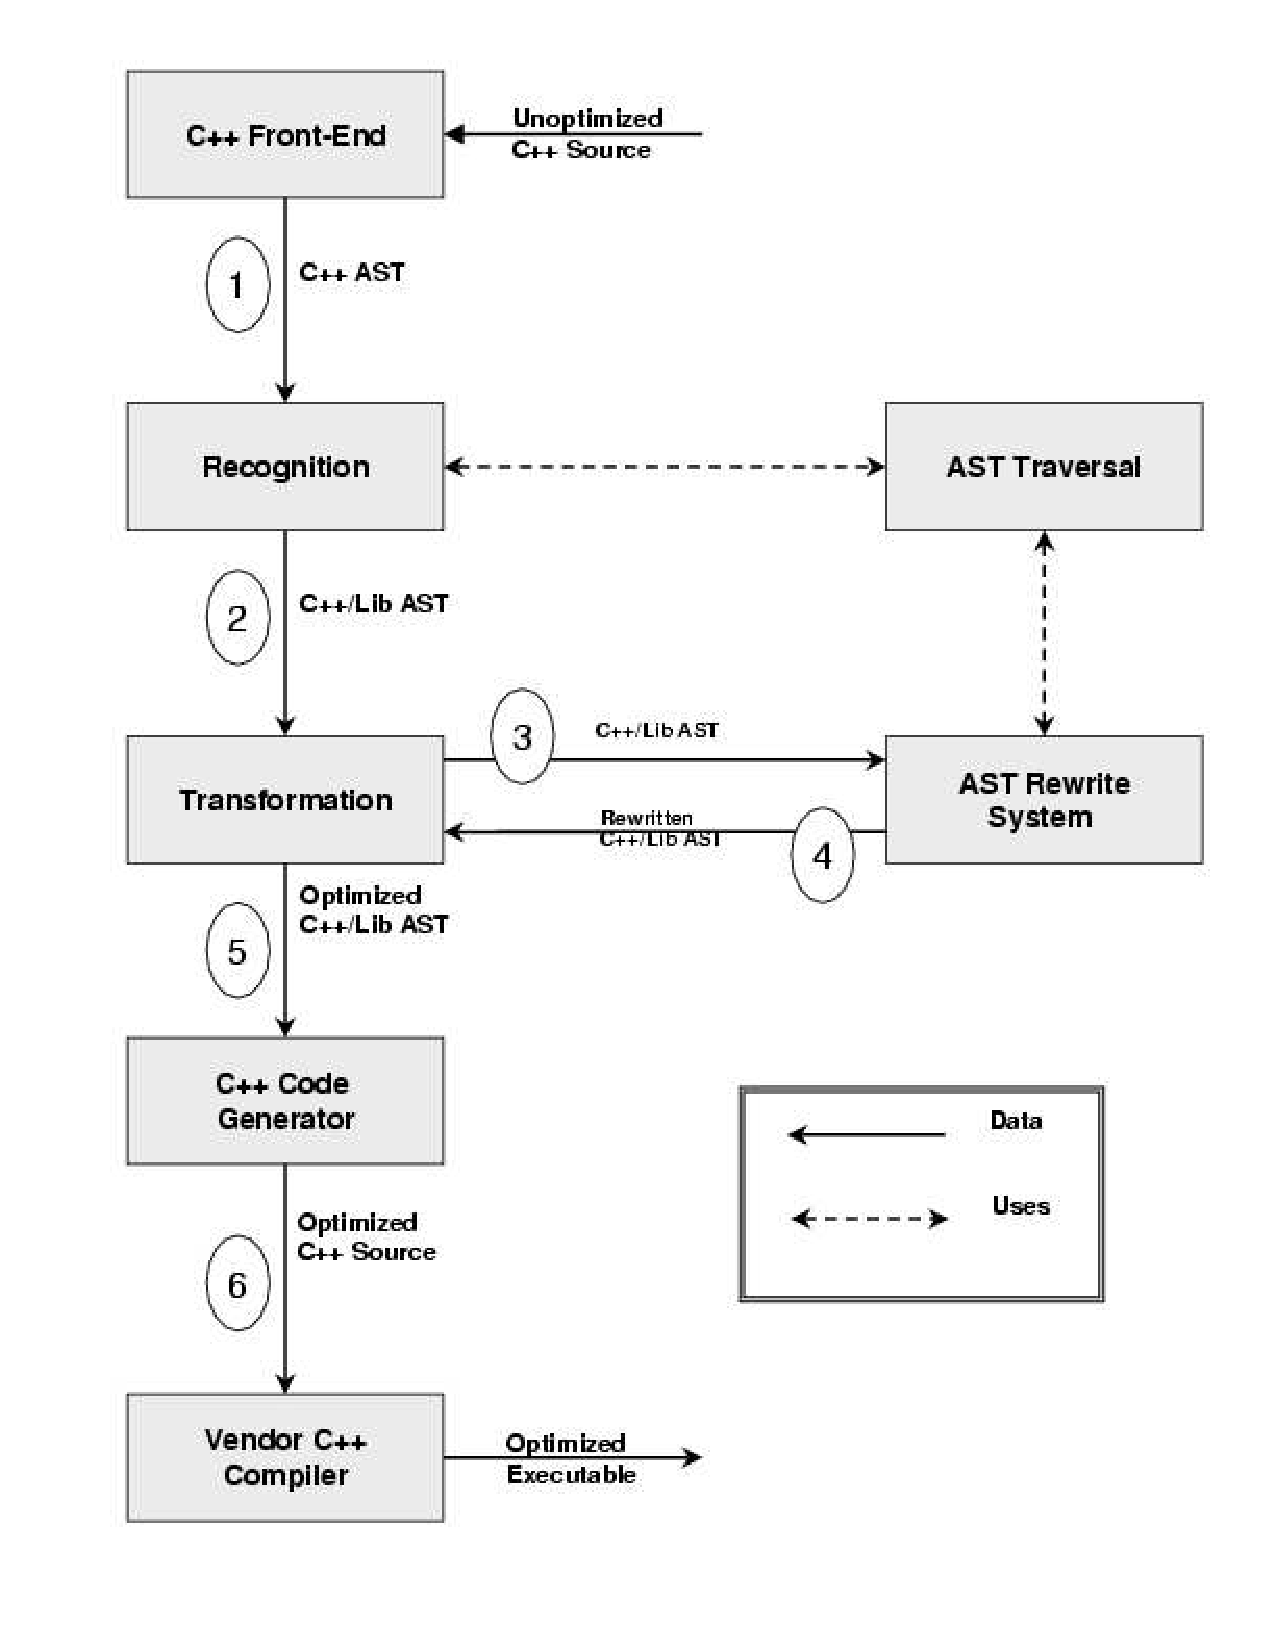
\psfig{file=rose-processing-phases.pdf,height=1.0\linewidth,width=1.0\linewidth,angle=0}}
%\centerline{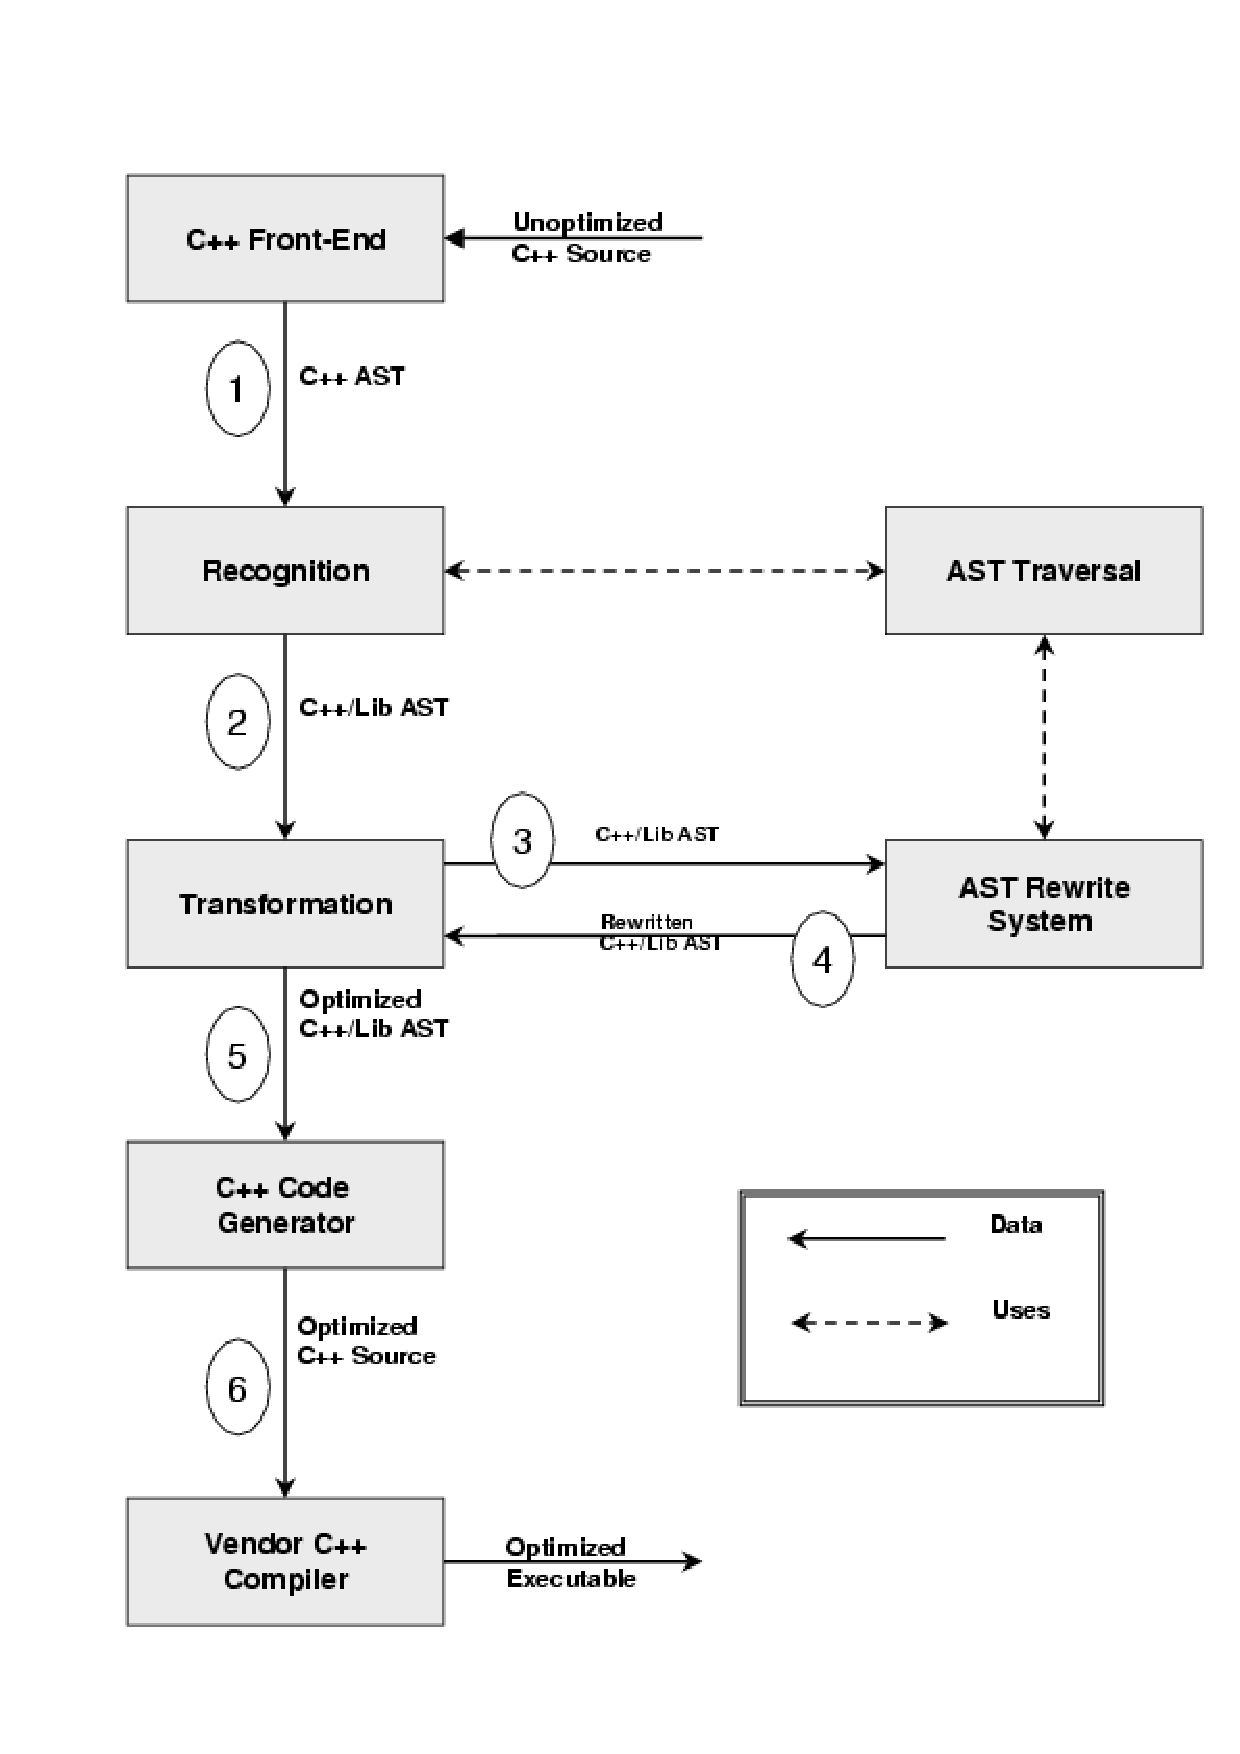
\includegraphics[height=1.0\linewidth,width=1.0\linewidth,angle=0]{rose-processing-phases}}
% \centerline{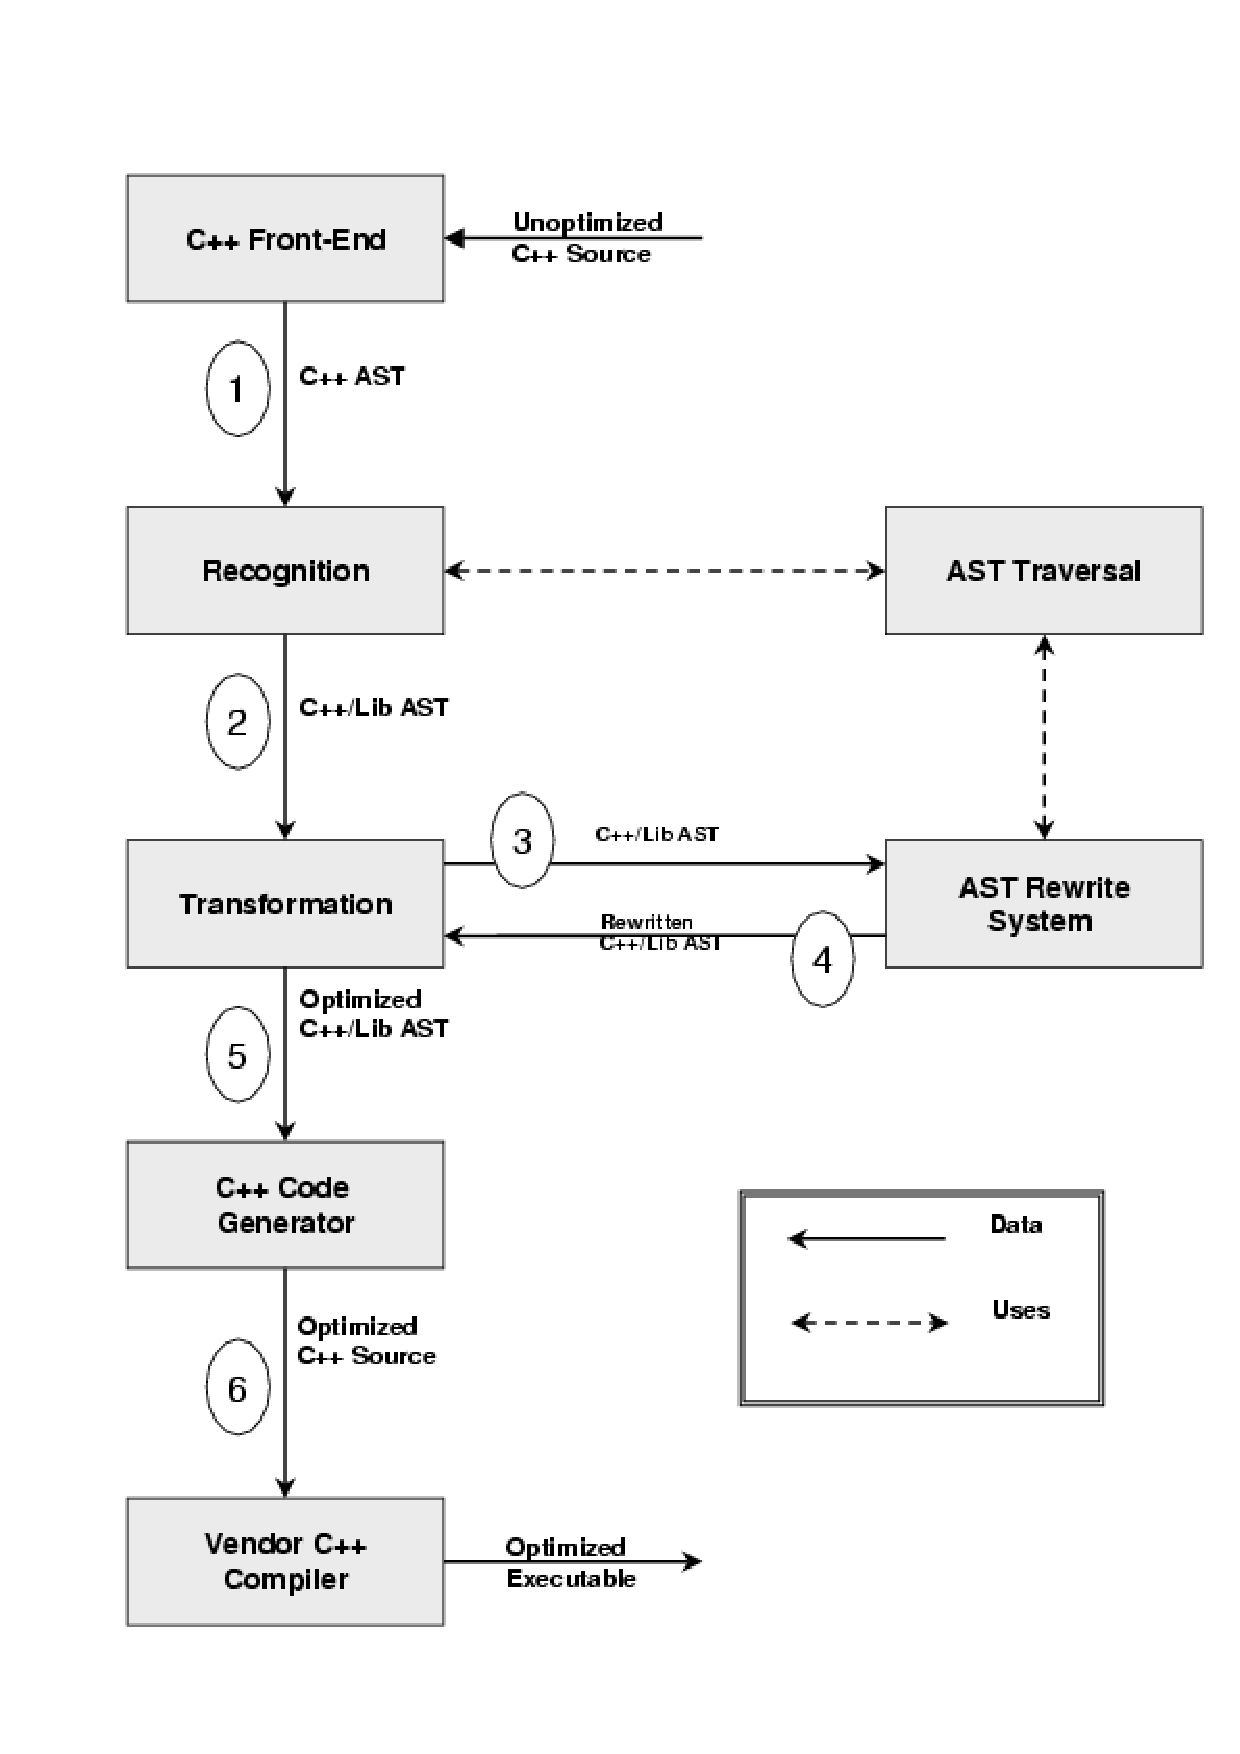
\includegraphics[height=1.0\linewidth,width=1.0\linewidth,angle=0]{rose-processing-phases}}
% the following line didn't work for me using acroread in Linux (tps 30Jun08) 
%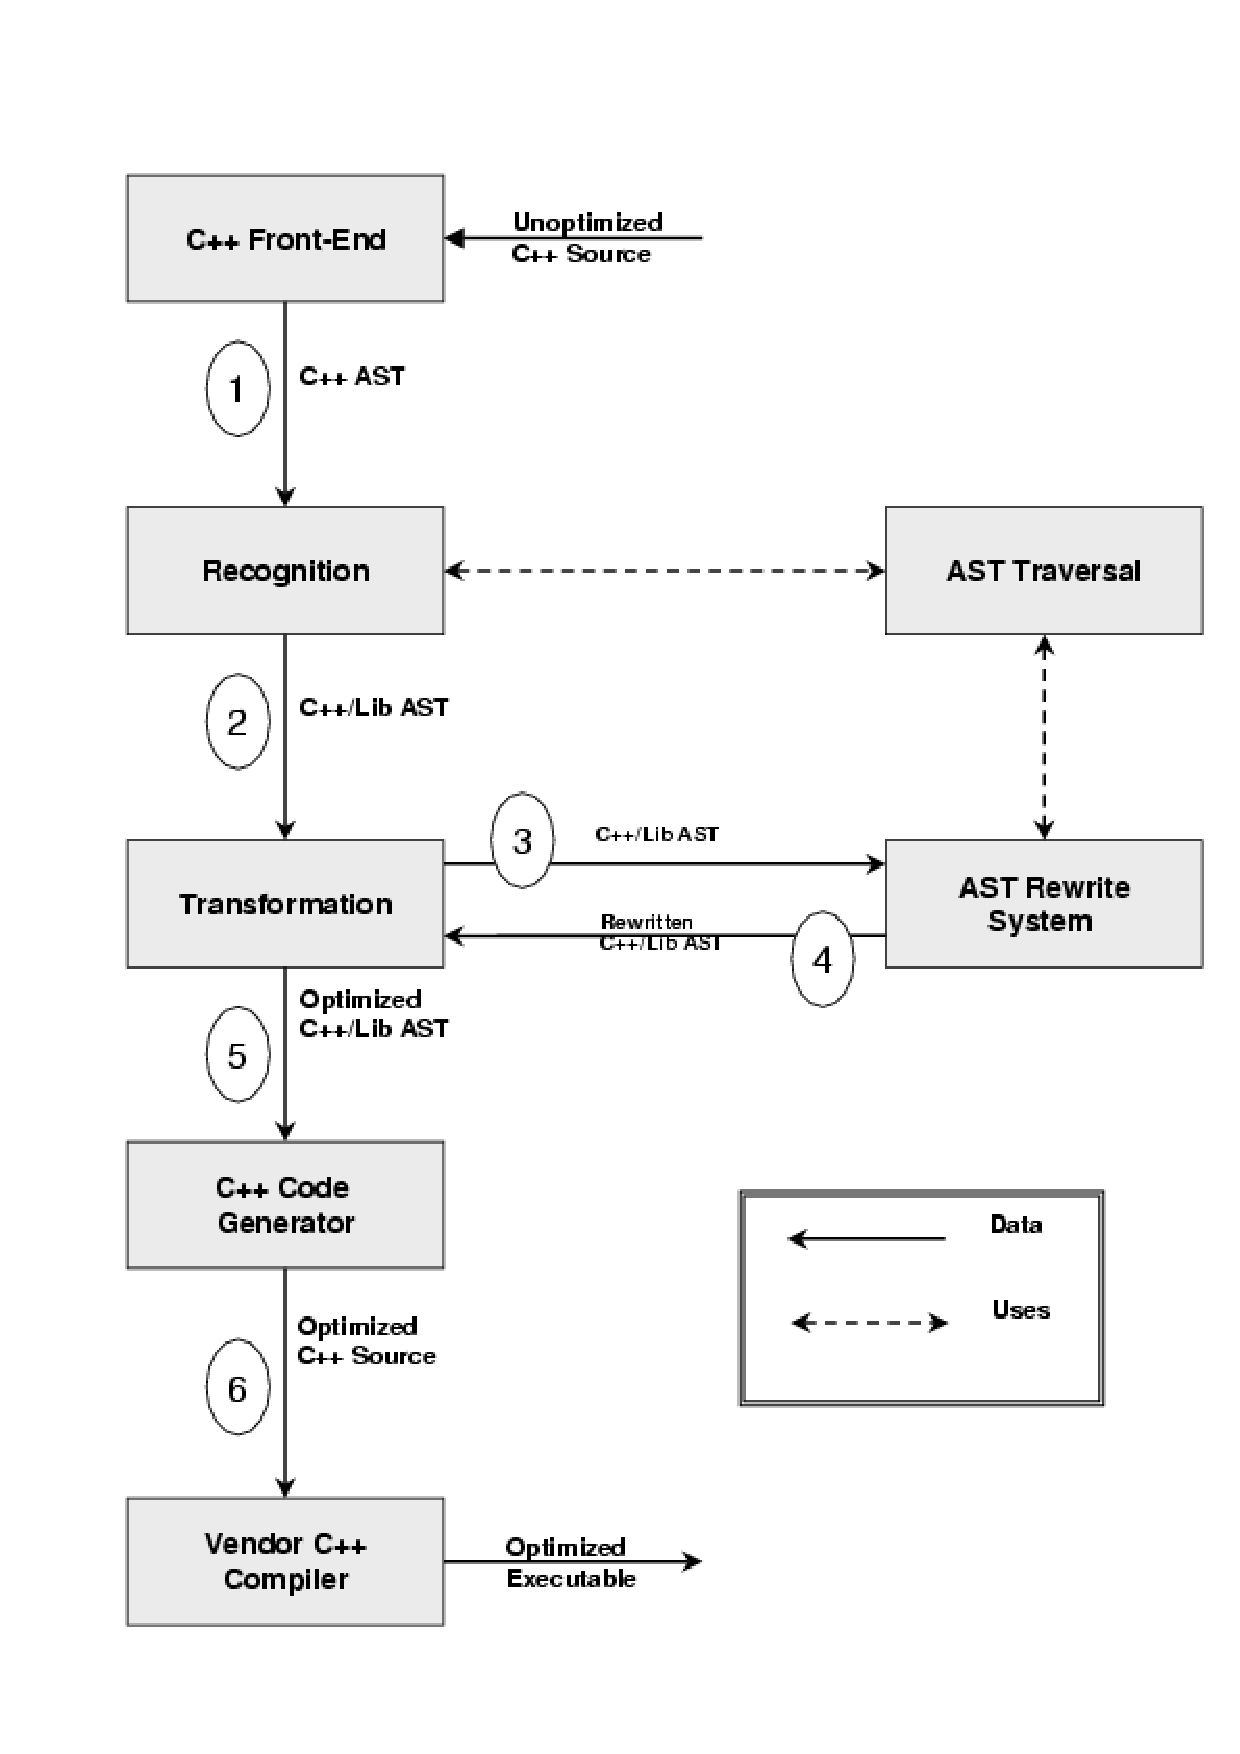
\includegraphics[trim=6.0in 0in 0in 0in,scale=0.5]{rose-processing-phases}
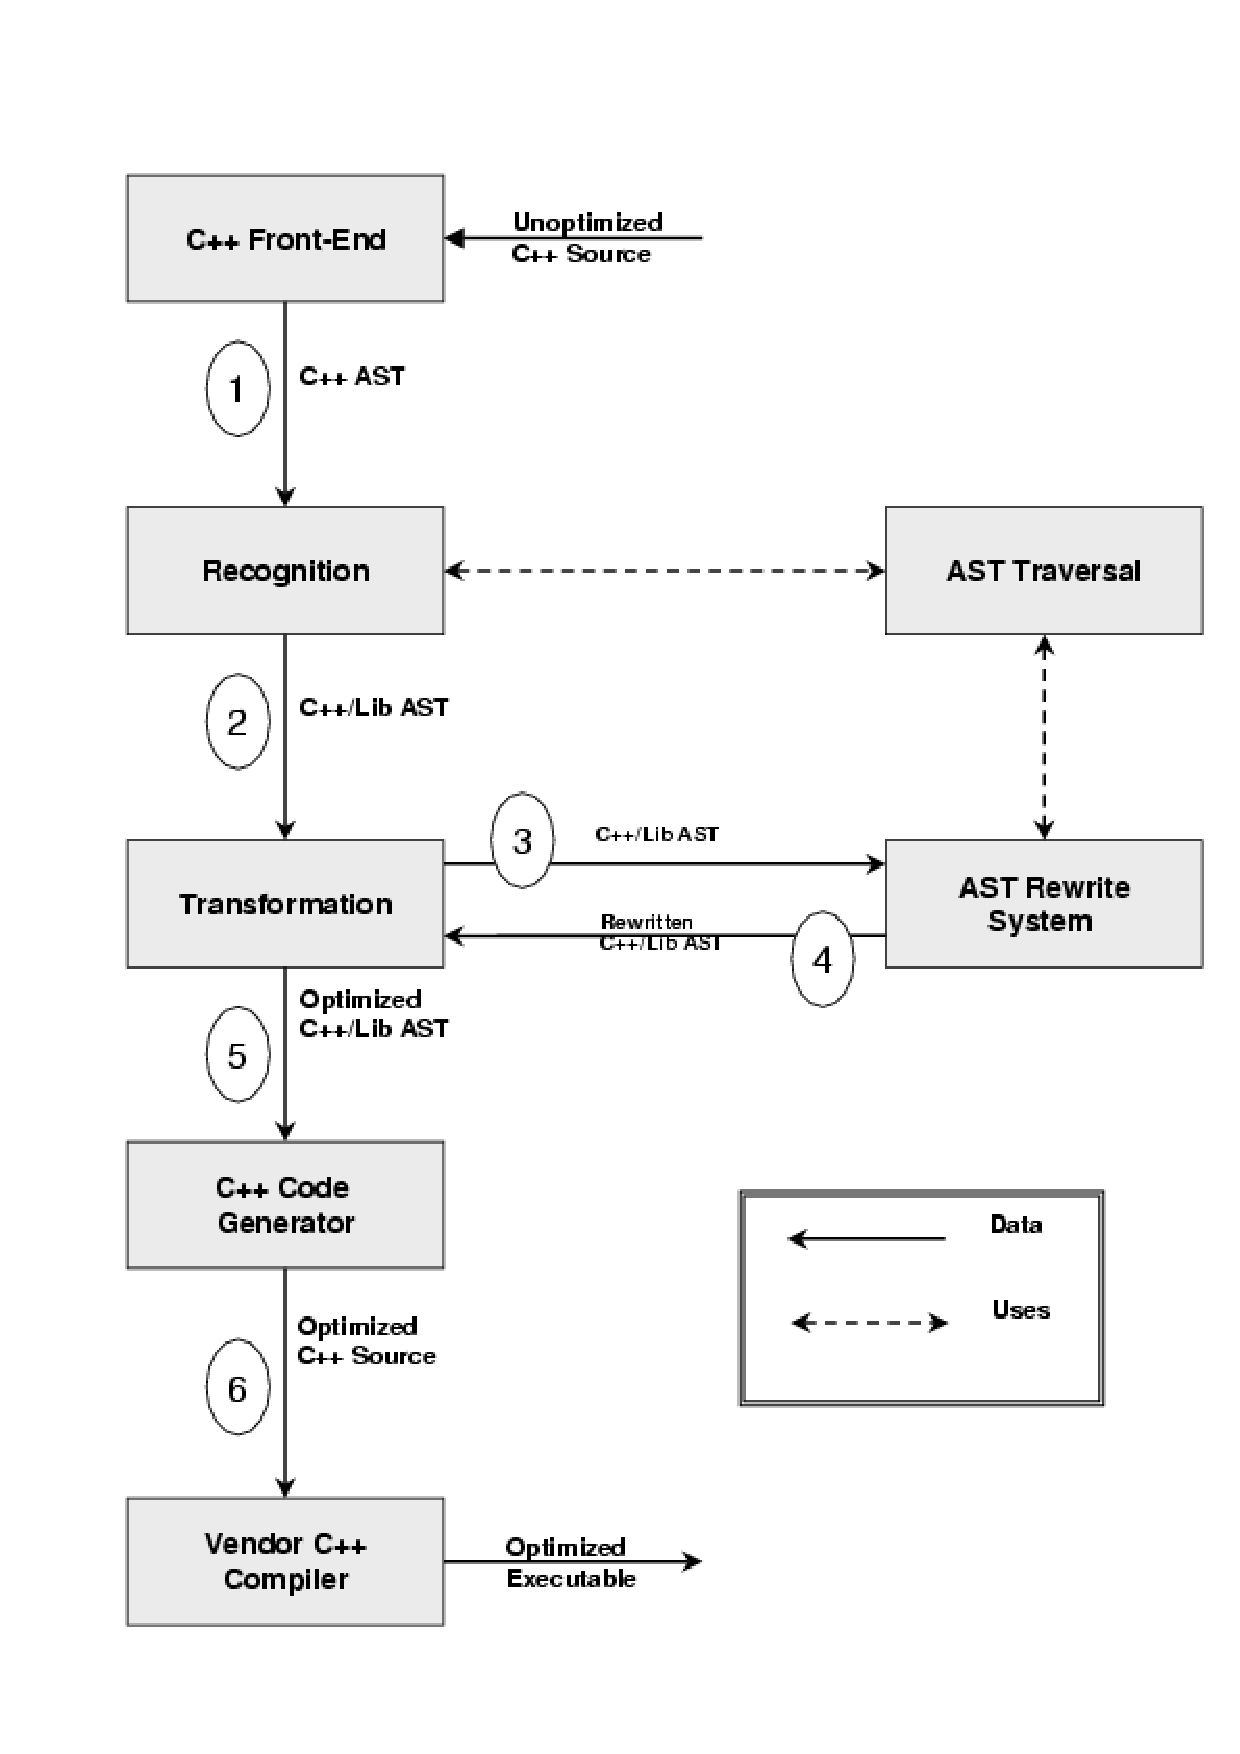
\includegraphics[scale=0.5]{rose-processing-phases}
\caption{Different phases of internal processing within translators built using ROSE infrastructure}
\label{introduction:phases}
\end{figure}



\section{ROSE Web Site}
    We have a ROSE Project Web page that can be accessed at the 
\htmladdnormallink{{\em ROSE}}{http://www.rosecompiler.org}
Web pages at
{\bf http://www.rosecompiler.org}.

This site is updated regularly with the latest documentation and software, as it is 
developed.
\footnote{All ROSE documentation is still in development}.


\section{ROSE Software/Documentation}
     ROSE is not yet released publicly on the Web, but is available
within the SciDAC Performance Evaluation Research Center (PERC) 
project and through limited collaborations with the developers
at universities and other laboratories.  Since the spring of 2006, we have made ROSE 
available via a password protected web page to all who have ask for access.
More information is available on the
\htmladdnormallink{ROSE}{http://www.rosecompiler.org} 
Web pages, located at:
{\bf http://www.rosecompiler.org}.
Web pages are updated regularly (postscript versions of 
documentation are available as well).

% When processing with latex2html use the -noinfo option to avoid generating
% a section ``About This Document'' which could be confused with this section.
\section{About This Manual}

   This section includes a description of what this manual
provides, how to use the manual, and the terminology related to
the examples.  
% Included in this introduction is 
An overview of the ROSE project is included. Error messages 
are contained in the Appendix (there are few at the moment).  
Further information is provided about
the ROSE Web site, where more information is available and where
the latest copy of the documentation is located.  This Web site will also be the
distribution site for ROSE, once it is made public; until then we welcome 
researchers to contact us directly to obtain pre-release versions of ROSE.

This manual is divided into several principal chapters.
Each chapter covers material that, in some cases, requires an understanding of
previous chapters. These are intended to simplify your use of this manual.
Each chapter is described briefly below:
\begin{itemize}
   \item {\bf Preface} \\
      This section briefly describes what this project is about.

   \item {\bf Acknowledgments} \\
      This section acknowledges contribution by many people over several years to the
      development of the ROSE project.

   \item {\bf Introduction} \\
      This chapter introduces why we have developed ROSE and some of its organization.

   \item {\bf Getting Started} \\
      This chapter walks the user through the configuration, compilation, installation,
      and testing of ROSE. Installation requirements are also explained. A small set of tests
      are available which verify the installation.

   \item {\bf Writing a Source-to-Source Translator} \\
      This chapter presents, by example, the details of writing a trivial translator using
      ROSE. 

   \item {\bf Overview of ROSE} \\
      This chapter presents details of specific features in ROSE.

   \item {\bf AST Query Library} \\
      This chapter presents work that has been completed to support simple and complex queries on the AST.

   \item {\bf AST Processing} \\
      This chapter covers different ways to write AST traversals (operators on the
      AST). This chapter 
    % requires an understanding of the previous chapter, and 
      is required to understand the subsequent chapter on the AST Rewrite Mechanism.

   \item {\bf AST Rewrite Mechanism} \\ This chapter covers the details of how to use the 
      mechanism within ROSE for modifying the AST. This chapter describes how to write
      general transformations on the Abstract Syntax Tree (AST).   It builds on concepts
      from the previous chapter.

   \item {\bf Program Analysis} \\
      This chapter explains what program analysis is available within ROSE.

   \item {\bf Loop Transformations} \\
      This chapter explains the loop optimization work that has been done.

   \item {\bf SAGE III Intermediate Representation} \\
      This chapter details issues specific to the IR used in ROSE.

   \item {\bf Appendix} \\ This contains information that has not yet made its way
      into the manual.  Much of this information will later be integrated into the 
      User Manual, but until then, it is provided for reference.  This chapter will at some point 
      contain a reference to error messages (there are few at present, most abort upon
      error, just like a compiler).

   \item {\bf Developer's Appendix} \\
      This chapter contains information specific to development of ROSE, and thus mostly 
    of use only for ROSE developers.

   \item {\bf Frequently Ask Questions (FAQ)} \\
      This chapter contains a series of frequently ask questions (FAQ) about the ROSE project.

   \item {\bf Glossary} \\ 
      Terms and definitions that simplify the documentation are included in this section. 
      More will be added over time.

\end{itemize}

   A later version of the manual will include performance data on different machines
so that the use of different features in ROSE can be better understood.  This
work is incomplete at present (implemented, but not yet represented in the documentation).










